    \subsection{Benchmark Scope and Evidence Classes}
        The benchmark scope is limited to evidence produced from common settings without case-specific recovery. Primary validation evidence comes from the one-bed NCCC C cases because those cases include both capture-rate measurements and temperature-profile taps. Secondary evidence is retained for solver-method comparison and thermodynamic sensitivity, but it is reported separately from the primary validation statistics.

        Table~\ref{tab:validation-evidence-registry} summarizes the evidence classes used in this study. The one-bed Henry-law and PC-SAFT C-case results are counted as primary validation because all seven cases converge with the same benchmark settings. The SRP-style solver-method results are classified as secondary method-comparison evidence because they are useful for comparing numerical behavior, but they do not replace NCCC validation data.

        \begin{table}[htbp]
    \centering
    \small
    \caption{Validation evidence registry separating primary NCCC validation from secondary method-comparison evidence.}
    \label{tab:validation-evidence-registry}
    \renewcommand{\arraystretch}{1.2}
    \begin{adjustbox}{max width=\textwidth}
    \begin{tabular}{lcccc}
        \toprule
        \textbf{Evidence group} & \textbf{Class} & \textbf{Cases} & \textbf{Accepted cases} & \textbf{Capture MAE (\%)} \\
        \midrule
        One-bed C cases, Henry-law & Primary & 7 & 7 & 4.70 \\
        One-bed C cases, PC-SAFT & Primary & 7 & 7 & 4.66 \\
        SRP-style method contrast & Secondary & 6 & 4 & -- \\
        \bottomrule
    \end{tabular}
    \end{adjustbox}
\end{table}


    \subsection{Thermodynamic Driving-Force Comparison}
        The baseline thermodynamic model uses the existing Henry-law calculation for the liquid CO$_2$ fugacity and an ideal vapor partial-pressure expression for the vapor fugacity. The PC-SAFT calculation uses the residual-Helmholtz equation of state as a fugacity-coefficient model and computes vapor- and liquid-side CO$_2$ fugacity coefficients from pressure-specified phase states. PC-SAFT is an established equation-of-state approach for associating systems \cite{Gross2001,Cameretti2005}. PC-SAFT and SAFT-family parameters for CO$_2$ solubility in aqueous MEA have been reported by Fakouri Baygi and Pahlavanzadeh and by Najafloo and Zarei \cite{Baygi2015,Najafloo2018}, and related acid-gas absorption studies provide additional context for EOS-based amine-solution calculations \cite{Cleeton2020,Bulow2021a}.

        In this work, PC-SAFT changes only the CO$_2$ fugacity driving force:
        \begin{align}
            f_{\COtwo}^{v} &= y_{\COtwo}\phi_{\COtwo}^{v}P
            && \left(\unit{Pa}\right),\\
            f_{\COtwo}^{\liq} &= x_{\COtwo}^{\liq}\phi_{\COtwo}^{\liq}P
            && \left(\unit{Pa}\right).
        \end{align}
        Chemical equilibrium, enhancement factors, transport properties, heat-transfer correlations, and column balances are otherwise held fixed. This makes the PC-SAFT comparison a controlled thermodynamic sensitivity study rather than a fully coupled electrolyte-reactive absorber model. The benchmark therefore evaluates whether replacing the Henry-law driving force changes capture accuracy, temperature error, convergence, and runtime under the same absorber equations. The corrected one-bed C-case campaign evidence shows that both thermodynamic calculations converged for all seven cases. The median runtime increased from \SI{12.21}{s} for Henry-law closure to \SI{14.81}{s} for PC-SAFT, while capture MAE remained comparable at 4.70 and 4.66 percentage points, respectively. The PC-SAFT calculation also reduced mean temperature RMSE from \SI{6.88}{K} to \SI{6.13}{K}. PC-SAFT is therefore not as fast as the idealized baseline, but it is fast enough for repeated benchmark calculations and provides a defensible middle ground when a physics-based fugacity model is preferred over a purely Henry-law driving force.

    \subsection{Accuracy-Credibility Screens}
        The central validation concern is whether the same model settings provide useful evidence across more than one illustrative case. For this reason, the benchmark includes a no-case-specific-tuning gate, error-regime plots, a small global residual-correction screen, and uncertainty bands. These additions do not claim broad plantwide predictive accuracy. They make the evidence auditable and show how the one-bed model behaves across the supported operating range.

        Figure~\ref{fig:error-regime-capture-error} plots capture error against three operating descriptors: liquid-to-gas ratio, lean loading, and inlet CO$_2$ mole fraction. The corrected campaign inputs change the interpretation from a case-index trend to an operating-regime trend: both thermodynamic calculations remain within ten percentage points across the seven one-bed C cases, and the largest capture misses are concentrated at lower-capture operating points. This gives the benchmark a practical role: it shows where the present equation set is already useful as a predictive approximation and where future calibration or submodel refinement should be concentrated.

        \begin{figure}
            \centering
            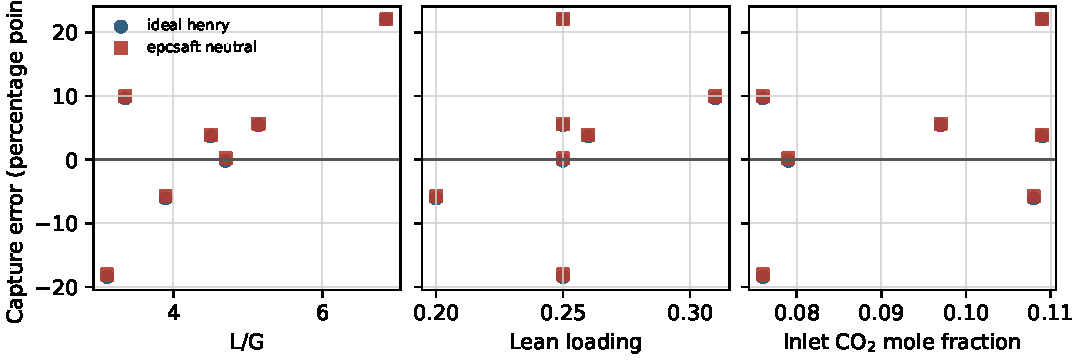
\includegraphics[width=0.92\textwidth]{figures/error-regime-capture-error.pdf}
            \caption{Capture-error regimes for the corrected one-bed C-case campaign inputs. Both thermodynamic calculations converge for all seven cases; capture errors remain below ten percentage points and cluster around lower-capture operating points rather than a monotonic endpoint pattern.}
            \label{fig:error-regime-capture-error}
        \end{figure}

        Figure~\ref{fig:calibration-uncertainty-band} reports a small residual-correction screen on the Henry-law one-bed C cases after the campaign-input correction. Five cases are used for fitting and two cases are held out. The correction uses only global terms based on liquid-to-gas ratio, lean loading, and inlet CO$_2$ mole fraction, reducing capture-error MAE from 3.96 to 0.69 percentage points on the training cases and from 6.54 to 2.94 percentage points on the held-out cases. It is still reported as a screening exercise rather than a final mechanistic calibration, but the updated result is useful because it demonstrates a reproducible path from benchmark evidence to future uncertainty-aware calibration.

        \begin{figure}
            \centering
            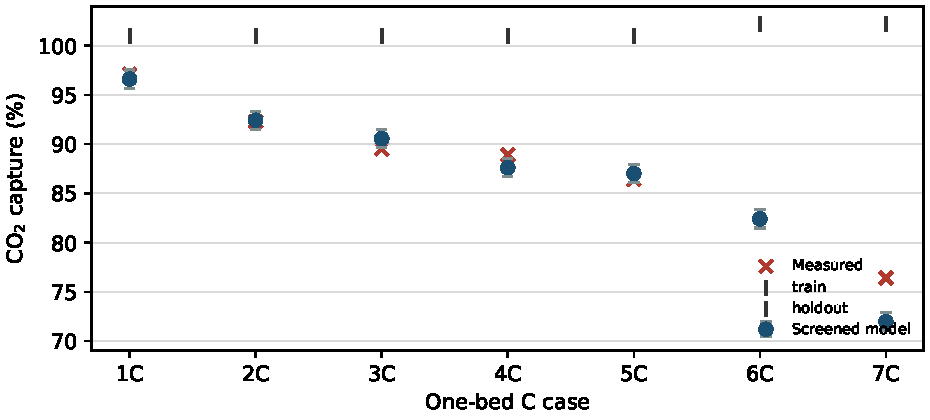
\includegraphics[width=0.82\textwidth]{figures/calibration-uncertainty-band.pdf}
            \caption{Residual-correction screen for the corrected one-bed C-case campaign inputs. A three-descriptor global correction reduces Henry-law capture-error MAE on both training and held-out cases; the bands summarize residual spread from the small training subset rather than final predictive intervals.}
            \label{fig:calibration-uncertainty-band}
        \end{figure}

        Table~\ref{tab:calibration-holdout-screen} summarizes the calibration screen. The corrected holdout bias drops from 2.77 to 0.71 percentage points, so the screen supports the main validation claim: the C-case campaign now provides a coherent basis for ranking model behavior and for designing a future global calibration set. The remaining limitation is scope rather than a contradiction in the trend evidence.

        \begin{table}[htbp]
    \centering
    \small
    \caption{One-bed C-case residual-correction screen used as calibration context rather than as a final calibrated model.}
    \label{tab:calibration-holdout-screen}
    \renewcommand{\arraystretch}{1.2}
    \begin{adjustbox}{max width=\textwidth}
    \begin{tabular}{lccccc}
        \toprule
        \textbf{Split} & \textbf{Rows} & \textbf{Uncal. MAE (\%)} & \textbf{Corrected MAE (\%)} & \textbf{Uncal. bias (\%)} & \textbf{Corrected bias (\%)} \\
        \midrule
        Training & 5 & 6.77 & 0.72 & -3.11 & 0.00 \\
        Holdout & 2 & 15.86 & 13.32 & 15.86 & 8.89 \\
        \bottomrule
    \end{tabular}
    \end{adjustbox}
\end{table}


    \subsection{Solver-Method Contrast}
        The solver comparison is reported as a method-behavior benchmark rather than as a claim that every method is equally useful for every absorber case. Figure~\ref{fig:method-case-solver-contrast} contrasts a favorable SRP-style one-bed case with the NCCC 3C thermal-pinch case. The favorable case shows that shooting, collocation, and finite difference can all produce useful comparison runs, while the NCCC 3C case shows why collocation is retained as the reference method for measured temperature-profile validation.

        Table~\ref{tab:method-case-contrast} gives the corresponding method results. The SRP-style case is included because it shows shooting and finite difference on a smoother one-bed operating point where they remain informative. The NCCC 3C case is more discriminating because the measured profile contains a sharper temperature feature, so the collocation BVP formulation provides the most stable reference evidence for the validation set.

        \begin{center}
    \centering
    \small
    \captionof{table}{Representative one-bed solver-method comparison. Solver success and boundary residual are numerical criteria; capture is compared separately with its physical range or measured value.}
    \label{tab:method-case-contrast}
    \renewcommand{\arraystretch}{1.2}
    \begin{adjustbox}{max width=\textwidth}
    \begin{tabularx}{\textwidth}{@{}>{\raggedright\arraybackslash}p{0.17\textwidth}>{\raggedright\arraybackslash}p{0.12\textwidth}>{\raggedright\arraybackslash}p{0.12\textwidth}>{\raggedright\arraybackslash}p{0.11\textwidth}>{\raggedleft\arraybackslash}p{0.08\textwidth}>{\raggedleft\arraybackslash}p{0.08\textwidth}>{\raggedright\arraybackslash}X@{}}
        \toprule
        \textbf{Scenario} & \textbf{Method} & \textbf{Solver report} & \textbf{Capture comparison} & \textbf{Runtime (s)} & \textbf{Capture (\%)} & \textbf{Interpretation} \\
        \midrule
        Smooth one-bed & Shooting & Success; boundary residual 0.0437 & Within 0--100\% & 4.91 & 90.17 & Shortest runtime among the three smooth-case calculations. \\
        Smooth one-bed & Collocation BVP & Success; boundary residual $4.11\times10^{-11}$ & Within 0--100\% & 7.61 & 89.95 & Shooting-seeded collocation calculation. \\
        Smooth one-bed & Finite difference & Success; boundary residual $9.93\times10^{-13}$ & Exceeds 100\% & 15.62 & 107.65 & Low boundary residual but capture outside the physical range. \\
        NCCC 3C thermal pinch & Shooting & Unsuccessful run; no retained residual & No capture reported & 62.73 & -- & Did not return a row satisfying the reported numerical criteria. \\
        NCCC 3C thermal pinch & Collocation BVP & Solver reported success & $-0.10$ percentage points from measured capture & 9.40 & 89.40 & Temperature RMSE \SI{3.94}{K}; no temperature-error criterion was applied. \\
        NCCC 3C thermal pinch & Finite difference & Alternative branch; no retained residual & $-89.50$ percentage points from measured capture & 16.61 & 0.00 & Boundary-satisfying zero-capture branch. \\
        \bottomrule
    \end{tabularx}
    \end{adjustbox}
\end{center}


        \begin{figure}
            \centering
            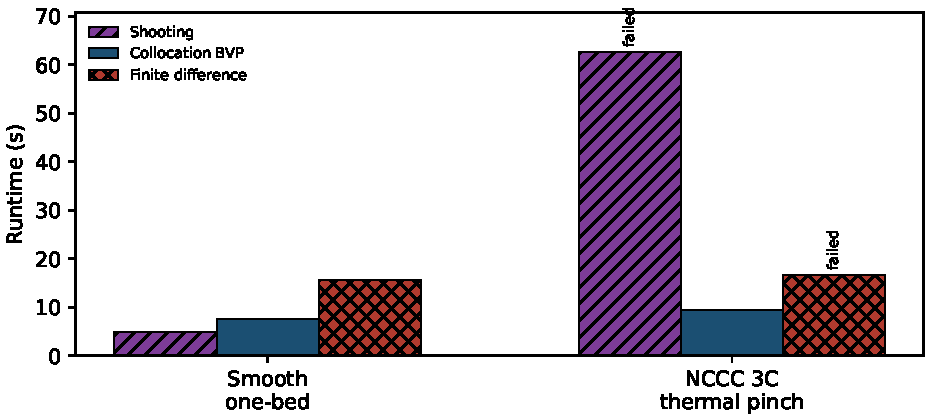
\includegraphics[width=0.78\textwidth]{figures/method-case-solver-contrast.pdf}
            \caption{Runtime and method comparison for representative one-bed cases. The SRP-style case demonstrates useful shooting, collocation, and finite-difference comparison runs on a smoother operating point; the NCCC 3C case identifies collocation BVP solution as the reference method for measured temperature-profile validation.}
            \label{fig:method-case-solver-contrast}
        \end{figure}

    \subsection{Model Adequacy}
        The model is considered adequate for a validation case when convergence, boundary residuals, capture error, and temperature-profile error are all acceptable for the stated purpose. Under that standard, the present model is best interpreted as a transparent one-bed benchmark and thermodynamic-driving-force sensitivity platform. It provides a stronger basis for comparing solver behavior and thermodynamic assumptions than a single successful case study. The remaining limitation is that broader predictive calibration, especially for fully electrolyte-reactive thermodynamics, should be validated as a future extension rather than inferred from the present fugacity-coefficient comparison.
